\documentclass{article}
\usepackage{graphicx}

\usepackage{booktabs}
\usepackage{makecell}
\usepackage{footnote} % footnote on table
\makesavenoteenv{tabular}
\makesavenoteenv{table}
\usepackage{longtable}

\begin{document}

\title{Spatial lag model with partial post sampling}
\author{}
\date{}
\maketitle

\section{Simulations}
\subsection{Simulation 1}
\begin{table}[h!]
    \begin{tabular}{cccccc}
      \toprule
        & 1Q & 2Q &3Q & 4Q \\
      \midrule
         NN & 1000 & 1200 & 500 & 100 \\
         nn & 70 & 30 & 150 & 50 \\
         $\beta$ & -2 & 10 & -5 & 3 \\
      \bottomrule
      \end{tabular}
      \end{table}

      \begin{table}[h!]
        \begin{tabular}{cl}
          \toprule
           Parameter & Values \\
          \midrule
             $\zeta$ &  0, 1, 2, 3, 4, 5\\
             $\lambda$  & 0.1, 0.3, 0.5, 0.7, 0.9 \\
          \bottomrule
          \end{tabular}
          \end{table}

\begin{figure}[p]
            \centering
            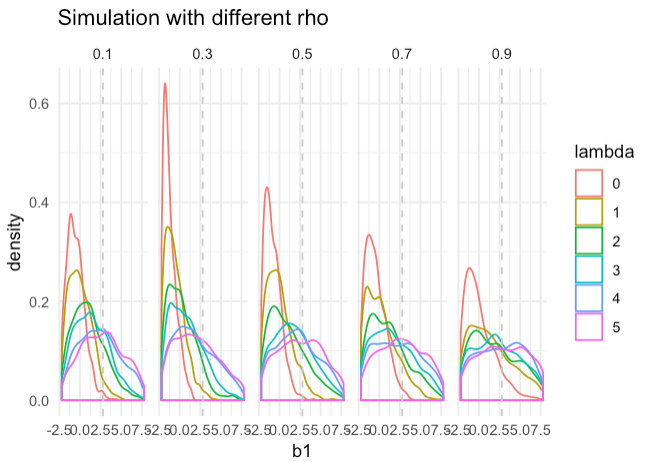
\includegraphics[width=\textwidth]{img/distribution1.png}
\end{figure}

\begin{figure}[p]
    \centering
    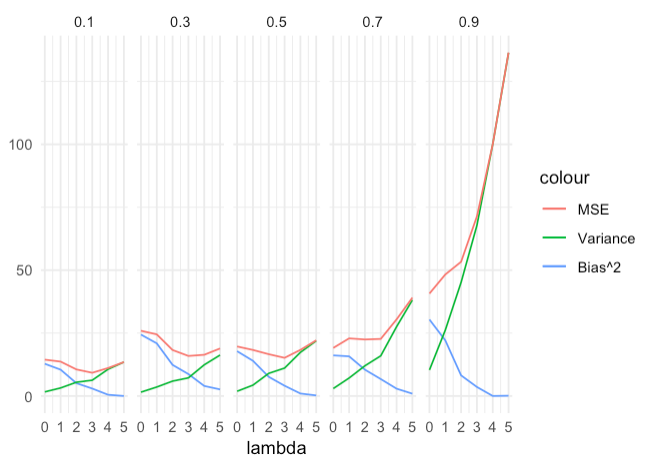
\includegraphics[width=\textwidth]{img/simulation1.png}
\end{figure}

\pagebreak 
\subsection{Simulation 2}
\begin{table}[!h]
    \begin{tabular}{cccccc}
      \toprule
        & 1Q & 2Q &3Q & 4Q \\
      \midrule
         NN & 1000 & 1200 & 500 & 100 \\
         nn & 70 & 30 & 150 & 50 \\
         $\beta$ & -2 & 2 & 5 & -3 \\
      \bottomrule
      \end{tabular}
      \end{table}

      \begin{table}[h!]
        \begin{tabular}{cl}
          \toprule
           Parameter & Values \\
          \midrule
             $\zeta$ &  0, 1, 2, 3, 4, 5\\
             $\lambda$  & 0.1, 0.3, 0.5, 0.7, 0.9 \\
          \bottomrule
          \end{tabular}
          \end{table}

\begin{figure}[p]
            \centering
            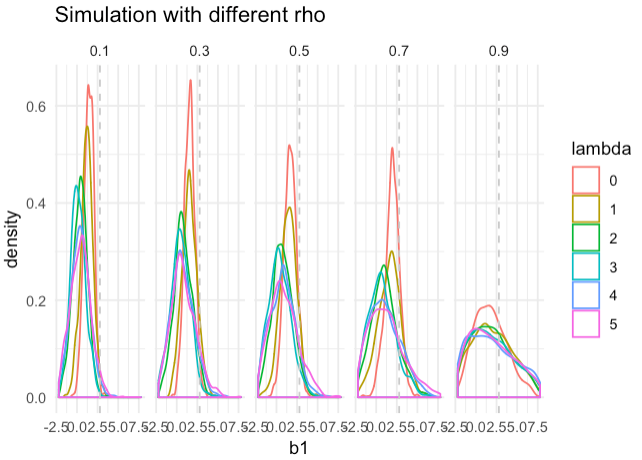
\includegraphics[width=\textwidth]{img/distribution2.png}
\end{figure}

\begin{figure}[p]
    \centering
    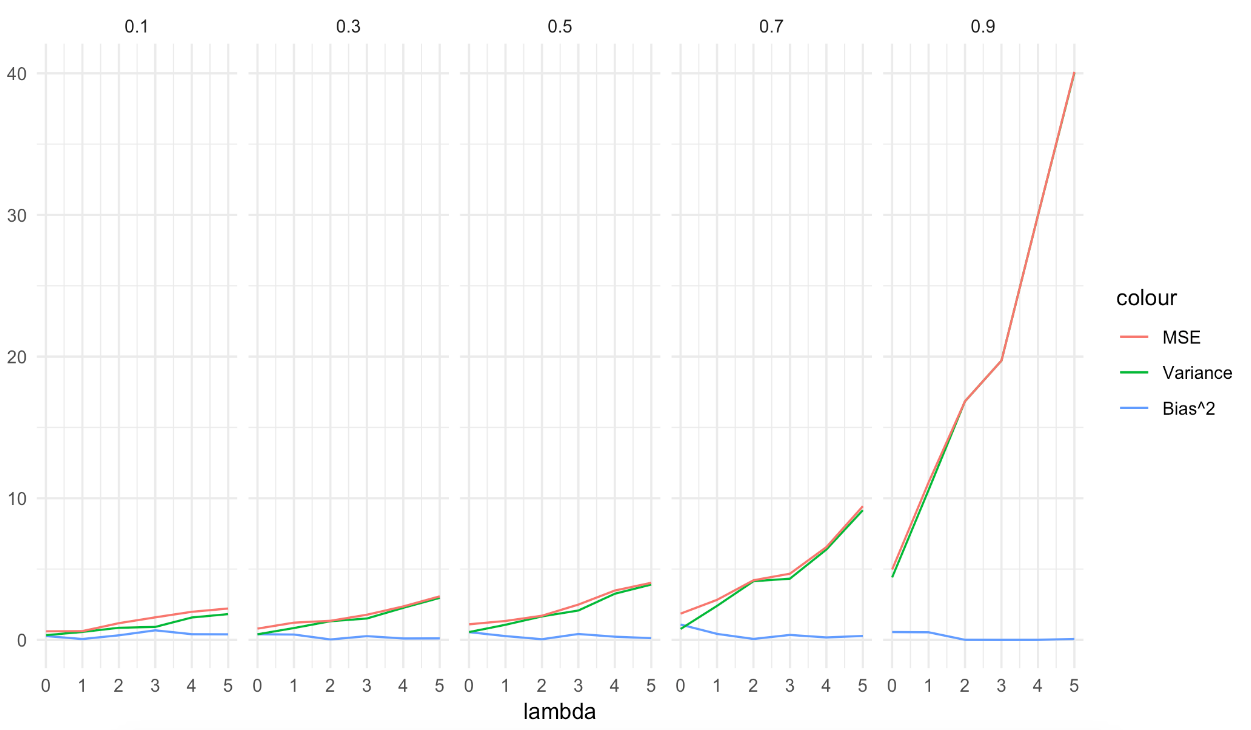
\includegraphics[width=\textwidth]{img/simulation2.png}
\end{figure}

\end{document}